\documentclass[a4paper]{article}
\usepackage[left=1.5cm,right=1.5cm]{geometry}
\usepackage{ctex}
\usepackage{graphicx}
\usepackage{siunitx}
\usepackage{float}
\usepackage{hyperref}
\usepackage{enumerate}
\usepackage[thehwcnt = 3]{iidef}
\thecourseinstitute{清华大学}
\thecoursename{计算机网络原理}
\theterm{2023年秋季学期}
\hwname{作业}
\begin{document}
\courseheader
\name{杨哲涵}
\section{PPPoE实验}
\begin{figure}[H]
    \centering
    \begin{minipage}[t]{0.45\linewidth}
        \centering
        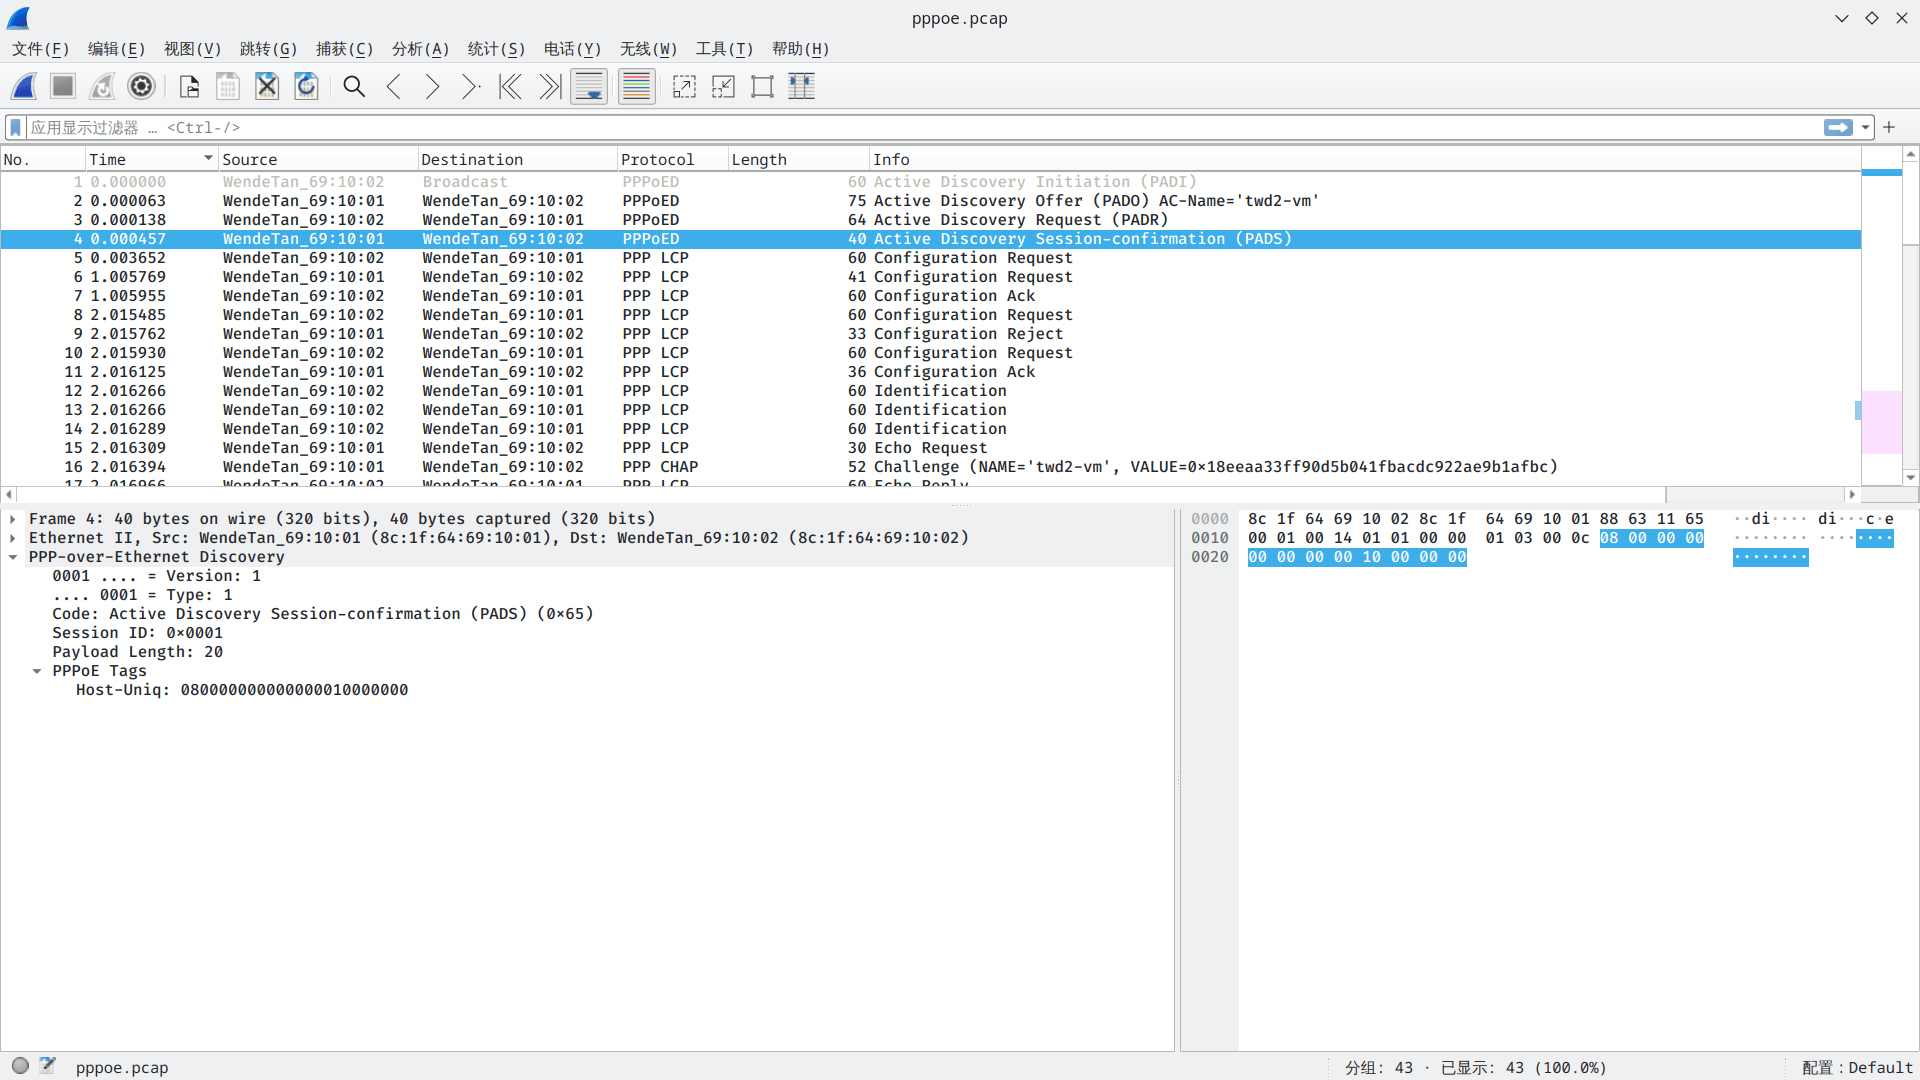
\includegraphics[width=\linewidth]{PPPoE-1.png}
        \caption{PADS}
        \label{1}
    \end{minipage}
    \begin{minipage}[t]{0.45\linewidth}
        \centering
        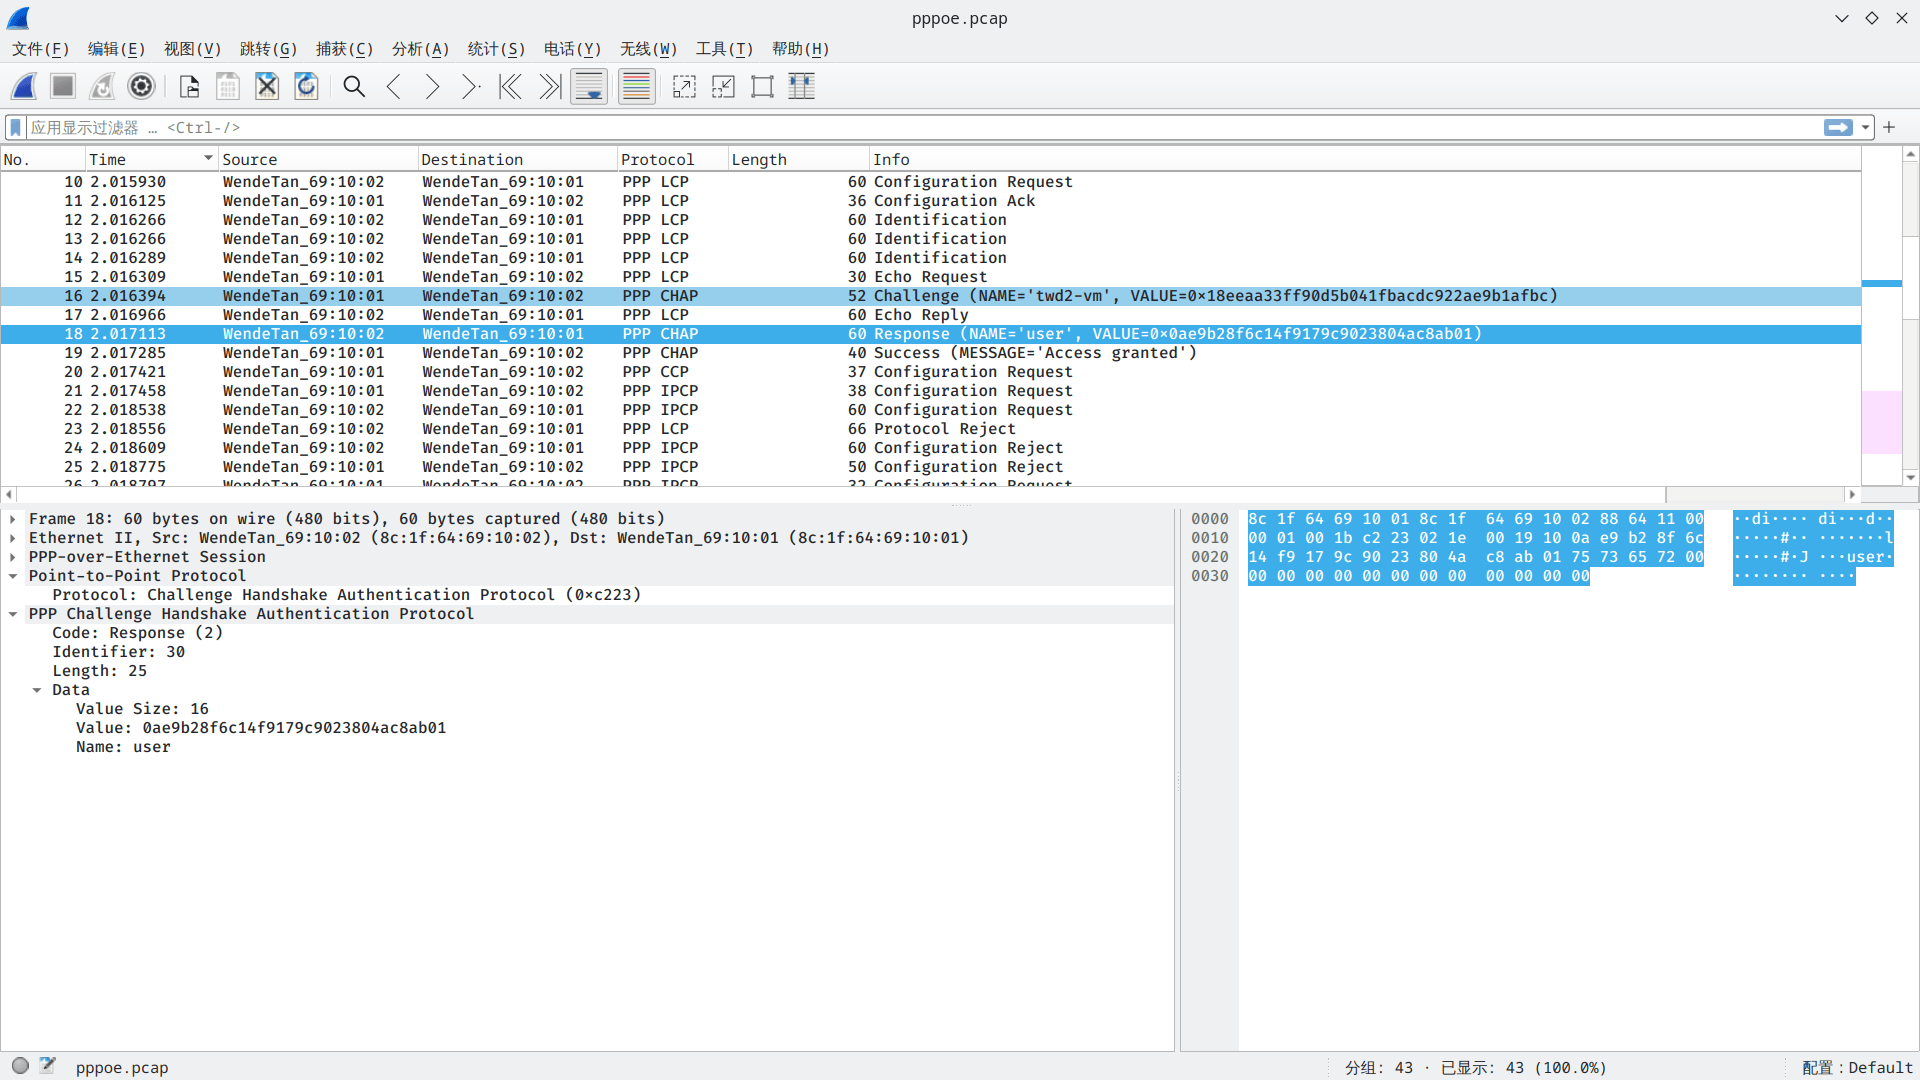
\includegraphics[width=\linewidth]{PPPoE-2.png}
        \caption{PPP CHAP Response}
        \label{2}
    \end{minipage}
    \begin{minipage}[t]{0.45\linewidth}
        \centering
        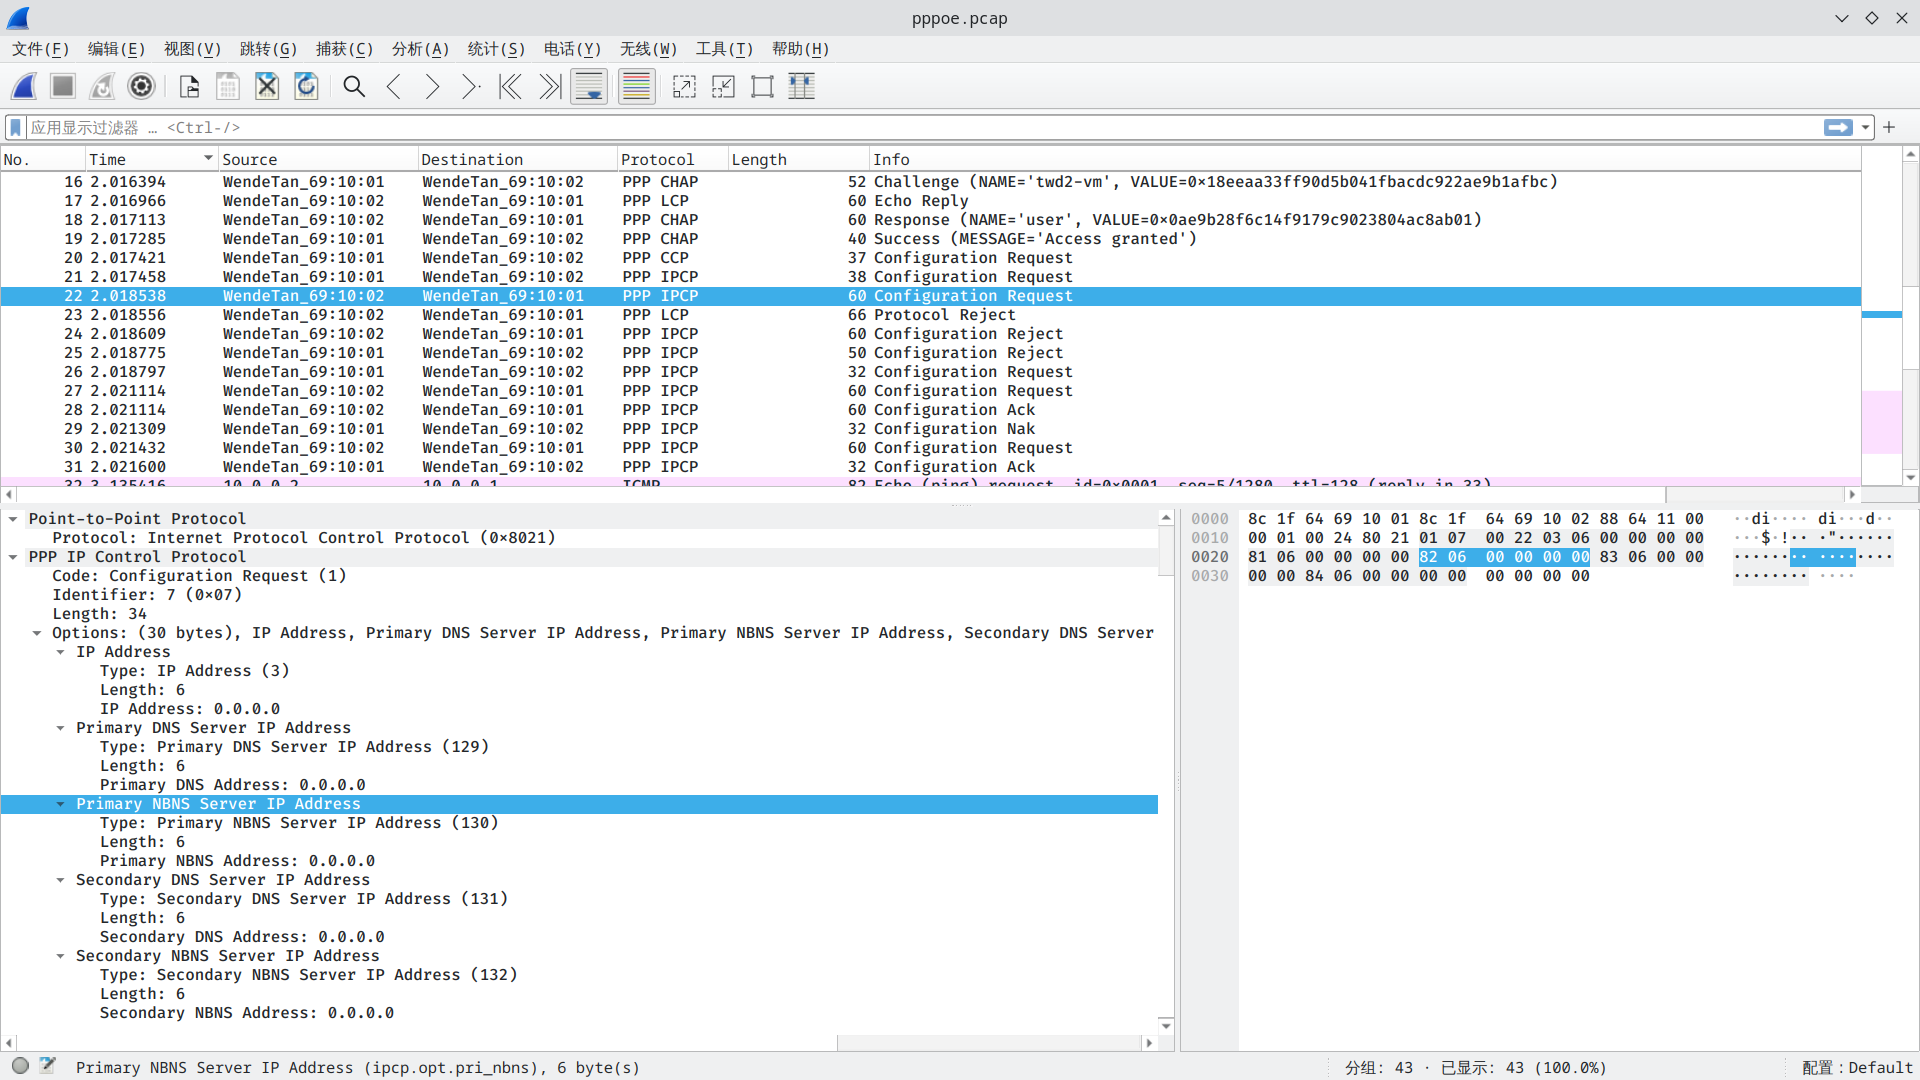
\includegraphics[width=\linewidth]{PPPoE-3.png}
        \caption{PPP IPCP Request}
        \label{3}
    \end{minipage}
    \begin{minipage}[t]{0.45\linewidth}
        \centering
        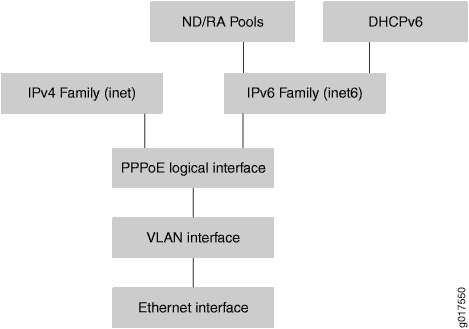
\includegraphics[width=\linewidth]{PPPoE-4.png}
        \caption{PPPoE双栈接入}
        \label{4}
    \end{minipage}
\end{figure}
PADS报文见图\ref{1}.PPPoE服务器的地址是\verb|8c1f64691001|,PPPoE客户端的地址是\verb|8c1f64691002|
\paragraph{2}
PPP CHAP Response与PPP IPCP Request报文见图\ref{2},\ref{3}.

PPP CHAP Response的加密摘要字段为\verb|0ae9b28f6c14f9179c9023804ac8ab01|.
\paragraph{3}
认为MTU即以太网DMAC,SMAC,Type后容纳的数据最多为1500字节.考虑PPPoE协议占用6个字节,PPP协议(PPPoE封装)占用2个字节,IPv4占用20个字节,UDP占用8个字节,那么上层应用能使用的最大容量为1464个字节.
\paragraph{4}
这是为了避免浪费字节.因为PPPoE中已经有VER,TYPE,CODE,SESSIONID字段.所以不必在PPP协议头中重复.
\paragraph{5}
MRU一般为1492字节,这是因为以太网MTU=1500字节,减去PPoE,PPP后为1492.此外MRU受到协商接受能力的限制.
\paragraph{6}
根据\url{https://www.juniper.net/documentation/cn/zh/software/junos/subscriber-mgmt-sessions/topics/topic-map/dual-stack-pppoe-access-monitoring-and-management.html},一种方案是IPv4与IPv6双栈共用PPPoE的逻辑接口,通过DHCPv6服务器解决IP地址分配的问题(参见图\ref{4}).这是一种兼容性很好的方案.
\paragraph{7}
PPPoE的优点是提供了一种身份验证方案,方便ISP提供商的计费,这种拨号上网方式非常流行.但是缺点在于需要额外的PPPoE服务器来管理,有额外冗余.现在有IPoE等技术,也有其他的不依赖PPPoE的准入管理方案(例如校园网).
\end{document}
